% !TEX root = 99_main.tex

\begin{figure}
\begin{center}
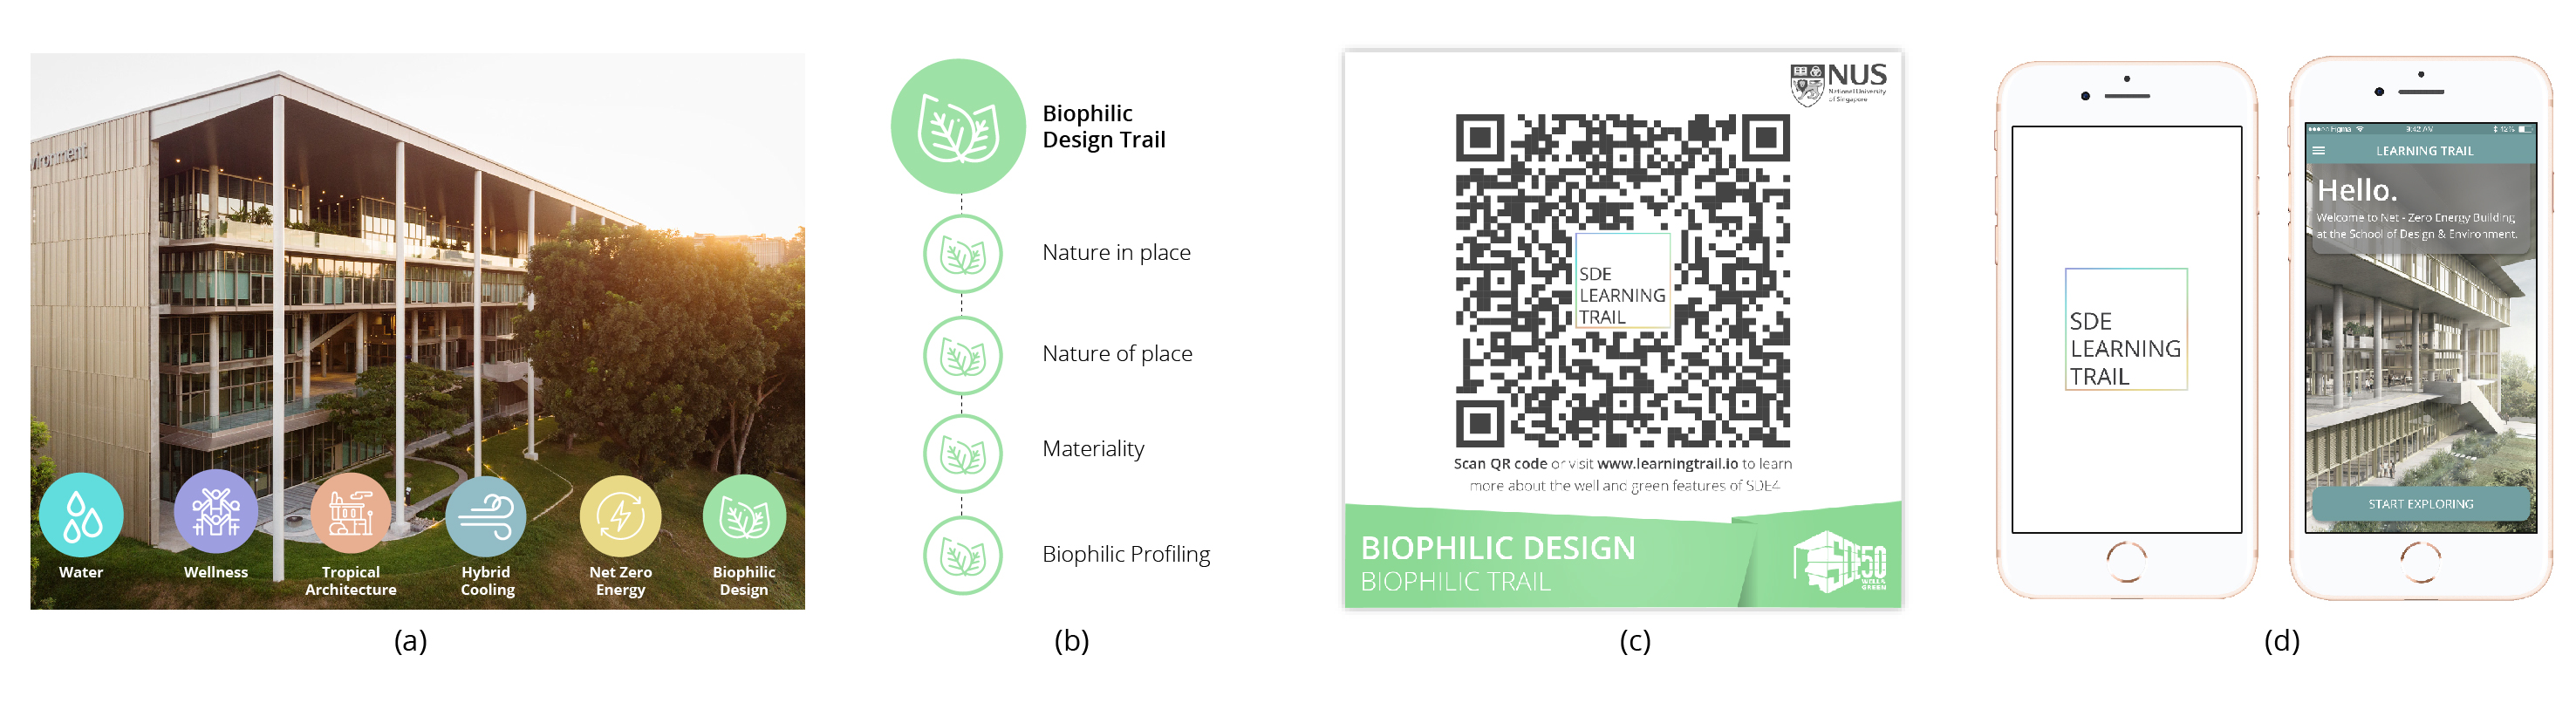
\includegraphics[width=\textwidth, trim= 0cm 0cm 0cm 0cm,clip]{Images/Fig1.jpg}
\caption{Overview of Experiment Setup: (a) Six building features described as trails, (b) Biophilic Design trail as an example of breaking down a trail into stations, (c) Biophilic Design trail as an example of trail placement in the building, (d) Digitisation of each physical station as a QR code.}
\label{fig:framework}
\end{center}
\end{figure}  

As shown in Figure \ref{fig:framework}, the SDE Learning Trail is a guided tour of the building's six different sustainability and wellness features - Net Zero Energy, Water, Hybrid Cooling, Wellness, Tropical Architecture, and Biophilic Design - as distinct \emph{trails} for users. Each trail is composed of a number of physical \emph{stations} - in the form of placards that include explanatory labels and text as well as a QR code. These stations are spatially placed such that they help break down and explain the interesting building features in more detail. The framework is realised as a simple mobile web application which connects each station (QR code) with information and interactive visualizations online. As users complete each trail by visiting different stations, the application collects comfort feedback for thermal, visual and aural variables while enabling users to learn and appreciate the design, construction, and sustainability innovations. An overview of the trails and their content can be found online\footnote{\url{http://learningtrail.me/}}.

A total of 35 stations (6 trails) were spread across the 6 floors of the SDE4. The placement of a trail in the building was based on where the building feature was most pronounced. For example, the water trail stations were placed next to the storm water feature, bio-retention basins and the detention tank for the building. These placements helped instantly contextualize the digital content of trails and stations with their physical location in the building. Stations were placed in proximity of fixed sensors measuring seven attributes in real-time: temperature, humidity, noise, light, carbon-dioxide, volatile organic compounds and presence. The stations were distributed across outdoor and indoor spaces based on trail configuration, station content, and proximity to fixed sensors. The interactive mobile web application was launched on January 30th, 2019 at the opening ceremony of the new NZEB. Over the next three months, staff and students from the university, external governmental, industrial and academic delegations were organized into groups to take guided tours of the building led by the research team from SDE.

Each participant in the guided tours used the interactive mobile application to go through trails as shown in Figure \ref{fig:mobileapp}. Users could scan stations with the help of an embedded QR code scanner in the application. The application was built such that each user was prompted to provide temperature, light and noise level feedback though a 3-point scale as shown in Figure\ref{fig:mobileapp}c. Each user was prompted five times out of all the stations they visited to provide feedback during the guided tour. A total of 616 users used the application over three months, with 79 users providing over at least five votes each, totaling 1163 environmental comfort feedback points. The data from the users and fixed sensors was aggregated using a cloud-based, time-series database - which served as a platform for data acquisition, storage and error detection. The combination of location-based user comfort feedback and fixed environmental sensor data allowed clustering analysis of personalized comfort profiles of users. These two data sources were merged through matching feedback location (spatially localized through QR code placement), time of feedback collection (timestamp) and user ID (through an in-built anonymous authentication method). 

\begin{figure}
\begin{center}
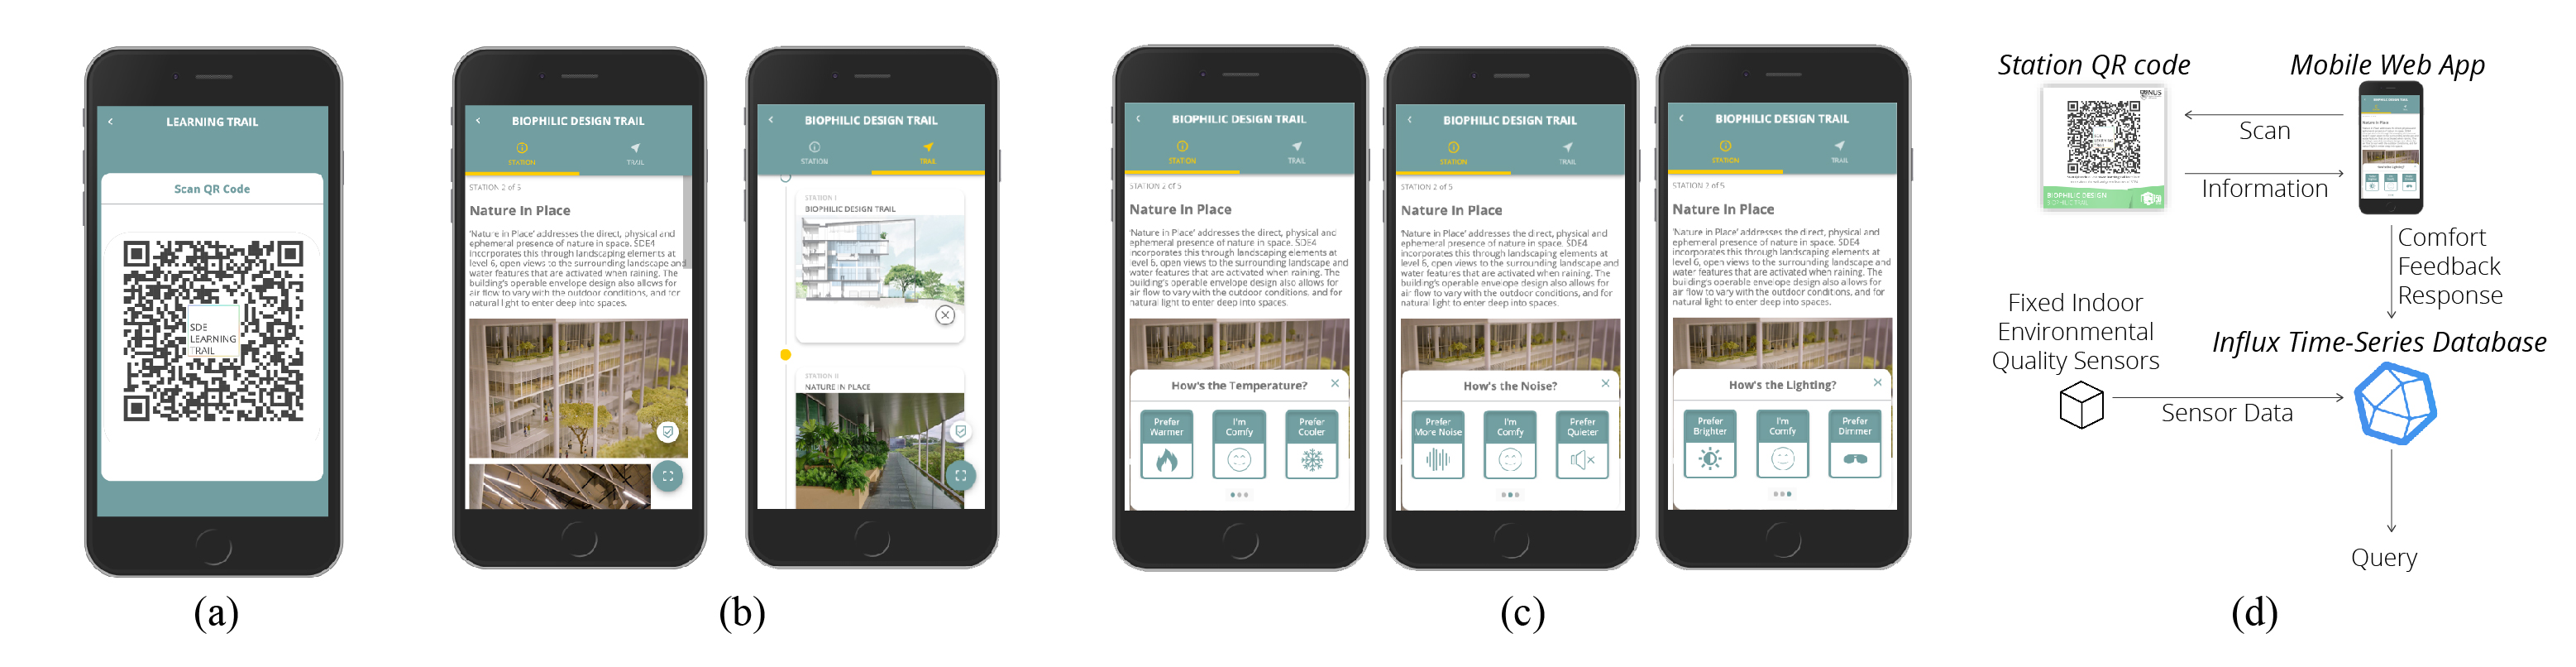
\includegraphics[width=\textwidth, trim= 0cm 0cm 0cm 0cm,clip]{Images/Fig2.jpg}
%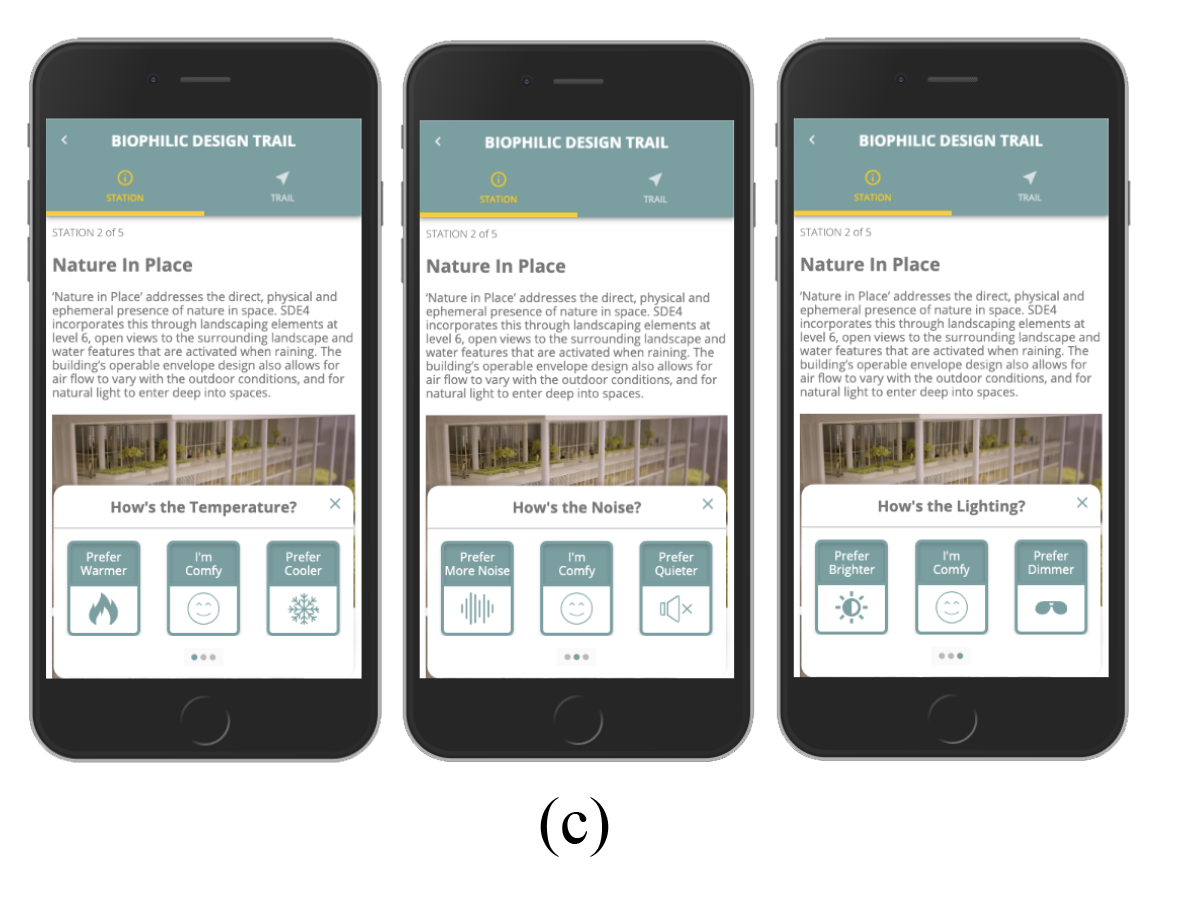
\includegraphics[width=\textwidth, trim= 0cm 0cm 0cm 0cm,clip]{Fig4.png}
\caption{Overview of the Learning Trail app: (a) The welcome screen and an inbuilt QR code scanner capability of the app, (b) Screens for sharing station content and trail configuration with the users, (c) In-built feedback prompts: Temperature - \emph{Prefer Warmer, Comfy, Prefer Cooler}, Light - \emph{Prefer Brighter, Comfy, Prefer Dimmer}, and Noise - \emph{Prefer Louder, Comfy, Prefer Quieter}, (d) Overview of data acquisition platform}
\label{fig:mobileapp}
\end{center}
\end{figure}

